\documentclass[11pt]{article}
\usepackage{amsmath, amssymb, mathtools, bm}
\usepackage{physics}
\usepackage{tikz}
\usepackage[margin=2.3cm]{geometry}
\usepackage{siunitx}
\usepackage{booktabs}
\usepackage{hyperref}
\usepackage{braket}

\newcommand{\de}{\mathrm{d}}
\newcommand{\pdone}[2]{\frac{\partial #1}{\partial #2}}
\newcommand{\pdtwo}[2]{\frac{\partial^{2} #1}{\partial #2^{2}}}
\newcommand{\Lap}{\nabla^{2}}
\renewcommand{\vb}[1]{\mathbf{#1}}

\title{B6 Condensed-Matter Physics --- Model Solutions, Trinity 2023\\
\large Paper A13485W1}
\author{}
\date{}

\begin{document}
\maketitle

\medskip
\noindent\emph{The candidate is required to attempt two questions out of four.  Below, full solutions to all four questions are provided in the Oxford lecturer style.}

%================================================================
\section*{Question 1 --- Neutron diffraction from \texorpdfstring{NaTaO$_3$}{NaTaO3}}

\textbf{Problem statement.}
The compound NaTaO$_3$ crystallises in a tetragonal lattice with $a=\SI{0.555}{nm}$, $c=\SI{0.393}{nm}$. The two-formula-unit cell contains two distinct oxygen sites with the fractional coordinates listed in the question; the four O$_2$ atoms are tilted by a small distortion parameter $\delta\ll 1$. We are asked to (a) derive the systematic-absence rule and the structure factor of Na, Ta, O$_1$ when $h+k=2n$; (b) expand the O$_2$ contribution to first order in $\delta$ for various parities of $h,k$; (c)~compute, for a powder neutron experiment with $\lambda=\SI{0.159}{nm}$ and resolution $\SI{0.05}{\degree}$ in $2\theta$, the squared structure factor, multiplicity and Bragg angle for the $(001)$, $(110)$ and $(210)$ reflections; (d) deduce $\delta$ from the measured intensities $I_{110}+I_{001}=1843$ and $I_{210}=345$.

\subsection*{(a) Systematic absences from Na, Ta, O$_1$}

The structure factor of an ion species $X$ occupying $N_X$ sites in the unit cell is
\begin{equation}
F_X(hkl)=b_X\sum_{j=1}^{N_X}\exp\!\bigl[2\pi i\bigl(hx_j+ky_j+lz_j\bigr)\bigr],
\label{eq:Fdef}
\end{equation}
where $(x_j,y_j,z_j)$ are the fractional coordinates of the $j$th atom of that species and $b_X$ is the neutron coherent scattering length.  Because the ions appear in pairs related by the centring vector $\bigl(\tfrac12,\tfrac12,0\bigr)$, the four sets of coordinates can be summed in pairs and a common phase $\exp\!\bigl[i\pi(h+k)\bigr]$ factored out.

For Na at $(0,\tfrac12,\tfrac12)$ and $(\tfrac12,0,\tfrac12)$,
\begin{equation}
F_{\mathrm{Na}}=b_{\mathrm{Na}}\,e^{i\pi l}\bigl[\,e^{i\pi k}+e^{i\pi h}\,\bigr].
\label{eq:Fna}
\end{equation}
For Ta at $(0,0,0)$ and $(\tfrac12,\tfrac12,0)$,
\begin{equation}
F_{\mathrm{Ta}}=b_{\mathrm{Ta}}\bigl[\,1+e^{i\pi(h+k)}\,\bigr].
\label{eq:Fta}
\end{equation}
For O$_1$ at $(0,0,\tfrac12)$ and $(\tfrac12,\tfrac12,\tfrac12)$,
\begin{equation}
F_{\mathrm{O1}}=b_{\mathrm{O}}\,e^{i\pi l}\bigl[\,1+e^{i\pi(h+k)}\,\bigr].
\label{eq:Fo1}
\end{equation}

If $h+k$ is odd, then $e^{i\pi(h+k)}=-1$, so equations \eqref{eq:Fta} and \eqref{eq:Fo1} vanish identically.  Equation \eqref{eq:Fna} is also zero, because $e^{i\pi k}=-e^{i\pi h}$ when $h$ and $k$ have opposite parity.  Hence \emph{none} of Na, Ta, O$_1$ contributes to a Bragg peak with $h+k=2n+1$.  This is the centring-rule absence of the body-centred sublattice that these three ions populate.

If $h+k=2n$ then $e^{i\pi h}=e^{i\pi k}=(-1)^h$, $e^{i\pi(h+k)}=+1$, and the three contributions sum to
\begin{equation}
\boxed{\,F_{\mathrm{Na+Ta+O1}}(hkl)=2\bigl[\,b_{\mathrm{Ta}}+b_{\mathrm{O}}(-1)^{l}+b_{\mathrm{Na}}(-1)^{h+l}\,\bigr]\quad (h+k=2n).\,}
\label{eq:Fmain}
\end{equation}
The pre-factor $2$ counts the two formula units in the cell, and the alternating signs reflect the relative axial offsets of Na ($z=\tfrac12$, plus a body-centring shift) and O$_1$ ($z=\tfrac12$).

\subsection*{(b) Structure factor of O$_2$ to first order in $\delta$}

The four O$_2$ ions all lie in the $z=0$ plane, so the $l$-dependent phase $e^{2\pi i l z}$ is unity for every term.  Writing the four positions as
\[
(\tfrac14+\delta,-\tfrac14+\delta,0),\;(-\tfrac14-\delta,\tfrac14-\delta,0),\;(\tfrac14-\delta,\tfrac14+\delta,0),\;(-\tfrac14+\delta,-\tfrac14-\delta,0),
\]
the corresponding phases factorise in a useful way: terms 1 and 2 are complex conjugates, and so are terms 3 and 4.  One finds
\begin{equation}
F_{\mathrm{O2}}=2b_{\mathrm{O}}\Bigl\{\cos\!\bigl[\tfrac{\pi}{2}(h-k)+2\pi\delta(h+k)\bigr]+\cos\!\bigl[\tfrac{\pi}{2}(h+k)+2\pi\delta(k-h)\bigr]\Bigr\}.
\label{eq:Fo2-exact}
\end{equation}
This expression is exact in $\delta$.  Expanding to first order using $\cos(\theta+\epsilon)\approx \cos\theta-\epsilon\sin\theta$,
\begin{equation}
\frac{F_{\mathrm{O2}}}{2b_{\mathrm{O}}}\!\approx\!\cos\!\tfrac{\pi(h-k)}{2}+\cos\!\tfrac{\pi(h+k)}{2}-2\pi\delta\!\left[(h+k)\sin\!\tfrac{\pi(h-k)}{2}+(k-h)\sin\!\tfrac{\pi(h+k)}{2}\right].
\label{eq:Fo2-lin}
\end{equation}
We now read off the three parity cases.

\paragraph{(i) $h$ and $k$ both odd.} Both $(h\pm k)/2$ are integers, so the two sines vanish.  The two cosines are $(-1)^{(h-k)/2}$ and $(-1)^{(h+k)/2}$; their indices differ by~$k$ (odd) and so have opposite parity.  Therefore
\begin{equation}
\boxed{\,F_{\mathrm{O2}}=0\quad(h,k\text{ both odd}).\,}
\label{eq:Fo2-oddodd}
\end{equation}
The two oxygen pairs contribute with opposite signs and cancel \emph{exactly} (not merely to first order) for these reflections.

\paragraph{(ii) $h$ and $k$ both even.} Again the sines vanish, and now $(h-k)/2$ and $(h+k)/2$ have the same parity (their difference is~$k$, an even integer).  The two cosines are equal, so
\begin{equation}
\boxed{\,F_{\mathrm{O2}}=4b_{\mathrm{O}}\,(-1)^{(h+k)/2}\quad(h,k\text{ both even}).\,}
\label{eq:Fo2-eveneven}
\end{equation}

\paragraph{(iii) One of $h,k$ even, the other odd.} Now $(h\pm k)/2$ are half-integers, so both cosines vanish; only the $\delta$-linear term survives.  Writing $s_1=(-1)^{(h-k-1)/2}$ and using $s_2/s_1=(-1)^k$:
\begin{itemize}
\item If $k$ is even (so $h$ odd): $s_2=s_1$, and \eqref{eq:Fo2-lin} gives $F_{\mathrm{O2}}=-2b_{\mathrm{O}}\cdot 4\pi\delta\,s_1\,k\cdot 0$\dots let us be careful. The combination is $[(h+k)+(k-h)]\,s_1 = 2k\,s_1$, hence
\begin{equation}
F_{\mathrm{O2}}=-8\pi\delta\,b_{\mathrm{O}}\,k\,s_1.
\label{eq:Fo2-keven}
\end{equation}
\item If $k$ is odd (so $h$ even): $s_2=-s_1$, giving
\begin{equation}
F_{\mathrm{O2}}=-8\pi\delta\,b_{\mathrm{O}}\,h\,s_1.
\label{eq:Fo2-kodd}
\end{equation}
\end{itemize}
In both cases the magnitude scales as $|\delta|\times(\text{the odd index})$, so these "mixed-parity" reflections appear \emph{only} because of the small O$_2$ tilt.  They are the diagnostic peaks for measuring $\delta$.

\subsection*{(c) Powder diffraction at $\lambda=\SI{0.159}{nm}$}

\paragraph{Lattice spacings.} Using the orthogonal-axes formula $d^{-2}=(h^2+k^2)/a^2+l^2/c^2$:
\begin{align}
d_{001}&=c=\SI{0.393}{nm},\\
d_{110}&=a/\sqrt{2}=\SI{0.555}{nm}/\sqrt2=\SI{0.39245}{nm},\\
d_{210}&=a/\sqrt{5}=\SI{0.555}{nm}/\sqrt5=\SI{0.24820}{nm}.
\end{align}

\paragraph{Bragg angles.} Solving $\sin\theta=\lambda/2d$:
\begin{align}
2\theta_{001}&=2\arcsin(0.159/0.786)=2\arcsin(0.20229)=\SI{23.34}{\degree},\\
2\theta_{110}&=2\arcsin(0.159/0.7849)=2\arcsin(0.20257)=\SI{23.38}{\degree},\\
2\theta_{210}&=2\arcsin(0.159/0.4964)=2\arcsin(0.32034)=\SI{37.36}{\degree}.
\end{align}
The separation $|2\theta_{110}-2\theta_{001}|\approx\SI{0.04}{\degree}$ is below the experimental resolution of $\SI{0.05}{\degree}$, so these two reflections merge into a single peak --- as advertised.

\paragraph{Structure factors.}  We use \eqref{eq:Fmain} together with the parity rules of part~(b).
\begin{itemize}
\item $(001)$: $h+k=0$ (even), $h$, $k$ both even. Equation \eqref{eq:Fmain} with $h=k=0,\,l=1$:
\begin{align}
F_{\mathrm{Na+Ta+O1}}&=2\bigl[b_{\mathrm{Ta}}-b_{\mathrm{O}}-b_{\mathrm{Na}}\bigr]=2(6.91-5.803-3.63)=\SI{-5.046}{fm}.
\end{align}
Equation \eqref{eq:Fo2-eveneven} with $(h+k)/2=0$ gives $F_{\mathrm{O2}}=4 b_{\mathrm{O}}=\SI{23.212}{fm}$.  Hence
\begin{equation}
F(001)=-5.046+23.212=\SI{18.166}{fm},\qquad |F(001)|^{2}\approx\SI{330}{fm^2}.
\end{equation}
\item $(110)$: $h+k=2$ (even), $h,k$ both odd. Using \eqref{eq:Fmain} with $h=k=1,\,l=0$,
\begin{equation}
F_{\mathrm{Na+Ta+O1}}=2\bigl[b_{\mathrm{Ta}}+b_{\mathrm{O}}-b_{\mathrm{Na}}\bigr]=2(6.91+5.803-3.63)=\SI{18.166}{fm},
\end{equation}
and \eqref{eq:Fo2-oddodd} gives $F_{\mathrm{O2}}=0$. Therefore
\begin{equation}
|F(110)|^{2}=(\SI{18.166}{fm})^{2}\approx\SI{330}{fm^2}.
\end{equation}
\item $(210)$: $h+k=3$ (odd), so by part~(a) the Na+Ta+O$_1$ contribution vanishes.  Only $F_{\mathrm{O2}}$ survives.  Here $h=2$ even, $k=1$ odd, so equation \eqref{eq:Fo2-keven} applies with $s_1=(-1)^{(h-k-1)/2}=(-1)^0=+1$:
\begin{equation}
F(210)=-8\pi\delta\,b_{\mathrm{O}}\,k\,s_1=-8\pi\delta\,b_{\mathrm{O}}=-8\pi\delta\cdot\SI{5.803}{fm},
\end{equation}
\begin{equation}
|F(210)|^{2}=64\pi^{2}\delta^{2}\,b_{\mathrm{O}}^{2}=64\pi^{2}\delta^{2}\cdot\SI{33.675}{fm^2}\approx 2.128\times 10^{4}\,\delta^{2}\,\si{fm^2}.
\end{equation}
\end{itemize}

\paragraph{Multiplicities for tetragonal symmetry.} The tetragonal point group $4/mmm$ generates the following equivalents:
\begin{itemize}
\item $(00l)$ family: only $(00\bar l)$ is symmetry-related; multiplicity $m_{001}=2$.
\item $(hh0)$ family with $h\ne 0$: the four members $(\pm h,\pm h,0)$; multiplicity $m_{110}=4$.
\item $(hk0)$ with $h\ne k\ne 0$: the eight members $(\pm h,\pm k,0)$ and $(\pm k,\pm h,0)$; multiplicity $m_{210}=8$.
\end{itemize}

Collecting:
\begin{center}
\begin{tabular}{lccc}
\toprule
$(hkl)$ & $|F|^{2}$ (fm$^{2}$) & multiplicity & $2\theta$\\
\midrule
$(001)$ & $330$ & $2$ & $\SI{23.34}{\degree}$\\
$(110)$ & $330$ & $4$ & $\SI{23.38}{\degree}$\\
$(210)$ & $\,\,2.13\times 10^{4}\,\delta^{2}$ & $8$ & $\SI{37.36}{\degree}$\\
\bottomrule
\end{tabular}
\end{center}
Since the $(001)$ and $(110)$ peaks are separated by only $\SI{0.04}{\degree}$ and the resolution is $\SI{0.05}{\degree}$, they cannot be resolved and appear as a single observed peak with combined intensity $I_{001}+I_{110}$.

\subsection*{(d) Determination of $\delta$}

The integrated powder intensity is $I_{hkl}=K\,m_{hkl}\,|F_{hkl}|^{2}$ with the same arbitrary scale factor $K$ for every reflection (geometrical Lorentz--polarisation factors having already been removed).  Because $|F(001)|^{2}=|F(110)|^{2}$, the merged peak satisfies
\begin{equation}
I_{001}+I_{110}=K\,(m_{001}+m_{110})\,|F(110)|^{2}=K\cdot 6\cdot 330\,\si{fm^2}=1980\,K\,\si{fm^2}.
\label{eq:I-sum}
\end{equation}
Setting this equal to the measured value~$1843$ fixes the scale,
\begin{equation}
K=1843/1980\,\si{fm^{-2}}\approx 0.9308\,\si{fm^{-2}}.
\label{eq:K-value}
\end{equation}
(In other words, the unit of intensity is $K^{-1}\approx 1.074\,\si{fm^{2}}$, but we shall not need this conversion separately.)

For the $(210)$ peak,
\begin{equation}
I_{210}=K\,m_{210}\,|F(210)|^{2}=K\cdot 8\cdot 64\pi^{2}\delta^{2}\,b_{\mathrm{O}}^{2}=512\pi^{2}\,K\,b_{\mathrm{O}}^{2}\,\delta^{2}.
\label{eq:I210}
\end{equation}
Inserting $b_{\mathrm{O}}^{2}=\SI{33.675}{fm^{2}}$, $K=0.9308$ and the measured $I_{210}=345$:
\begin{equation}
\delta^{2}=\frac{345}{512\pi^{2}\cdot 0.9308\cdot 33.675}=\frac{345}{1.583\times 10^{5}}=2.18\times 10^{-3}.
\end{equation}
Hence
\begin{equation}
\boxed{\,\delta\approx 0.047.\,}
\label{eq:delta-value}
\end{equation}
This is small enough ($\delta\ll 1$) for the linearisation \eqref{eq:Fo2-lin} to be self-consistent, and corresponds to an oxygen displacement of $\delta a\approx \SI{2.6e-2}{nm}\approx \SI{0.26}{\angstrom}$ --- a typical octahedral-tilt amplitude in perovskite-related compounds.

%================================================================
\section*{Question 2 --- Molecular orbital theory of H$_2$}

\textbf{Problem statement.} Two identical atoms (sites $1$ and $2$) carry single-particle orbitals $\ket{1}, \ket{2}$ of energy $\epsilon_0$, with $(\hat K+\hat V_i)\ket i=\epsilon_0\ket i$.  A trial wavefunction $\ket\psi=c_1\ket1+c_2\ket2$ is used in the variational quotient $\lambda=\bra\psi\hat H\ket\psi/\braket{\psi|\psi}$ for the two-atom Hamiltonian $\hat H=\hat K+\hat V_1+\hat V_2$.  The four matrix elements $V_{c1}=\bra2\hat V_1\ket2$, $V_{c2}=\bra1\hat V_2\ket1$, $t=-\bra1\hat V_2\ket2$ and $\sigma=\braket{1|2}$ are not assumed small, and overlap is retained.

\subsection*{(a) Secular equation without zero-overlap}

The numerator and denominator of $\lambda$ are
\begin{align}
N(c_1,c_2)&\equiv\bra\psi\hat H\ket\psi=\sum_{ij}c_i^{*}c_j H_{ij},\quad H_{ij}\equiv\bra i \hat H\ket j,
\label{eq:N}\\
D(c_1,c_2)&\equiv\braket{\psi|\psi}=\sum_{ij}c_i^{*}c_j S_{ij},\quad S_{ij}\equiv\braket{i|j}.
\label{eq:D}
\end{align}
We compute the four matrix elements explicitly.  For the diagonal entries, use $(\hat K+\hat V_1)\ket 1=\epsilon_0\ket 1$ to write $\hat H\ket 1=\epsilon_0\ket 1+\hat V_2\ket 1$, hence
\begin{equation}
H_{11}=\bra1\hat H\ket1=\epsilon_0+\bra1\hat V_2\ket1=\epsilon_0+V_{c2},\qquad H_{22}=\epsilon_0+V_{c1}.
\label{eq:Hdiag}
\end{equation}
For the off-diagonal entries, the same trick gives $\hat H\ket 2=(\hat K+\hat V_2)\ket2+\hat V_1\ket2=\epsilon_0\ket2+\hat V_1\ket2$, so
\begin{equation}
H_{12}=\bra1\hat H\ket2=\epsilon_0\sigma+\bra1\hat V_1\ket2.
\label{eq:H12-int}
\end{equation}
The remaining integral is converted via Hermiticity: $\bra1\hat V_1\ket2=\bra2\hat V_1\ket1^{*}$, and writing $\hat H\ket 1=\epsilon_0\ket 1+\hat V_2\ket 1$ gives $\bra 2 \hat H\ket 1=\epsilon_0\sigma^{*}+\bra2\hat V_2\ket1=\epsilon_0\sigma^{*}-t^{*}$. Therefore $H_{12}=\epsilon_0\sigma-t$, and similarly $H_{21}=\epsilon_0\sigma^{*}-t^{*}$.  In matrix form
\begin{equation}
\mathsf H=\begin{pmatrix}\epsilon_0+V_{c2}&\epsilon_0\sigma-t\\\epsilon_0\sigma^{*}-t^{*}&\epsilon_0+V_{c1}\end{pmatrix},\qquad
\mathsf S=\begin{pmatrix}1&\sigma\\\sigma^{*}&1\end{pmatrix}.
\label{eq:HS-mat}
\end{equation}

The condition for an extremum of $\lambda=N/D$ is $D\,\partial N/\partial c_i^{*}-N\,\partial D/\partial c_i^{*}=0$, i.e.\ at the extremum
\begin{equation}
\pdone{N}{c_i^{*}}=\lambda\,\pdone{D}{c_i^{*}}\quad\Longleftrightarrow\quad\sum_{j}H_{ij}c_j=\lambda\sum_{j}S_{ij}c_j.
\label{eq:secular}
\end{equation}
Here we used the formal independence of $c_i$ and $c_i^{*}$ (equivalently, varying real and imaginary parts independently).  Putting this in matrix notation and rearranging,
\begin{equation}
\boxed{\,(\mathsf H-\lambda\mathsf S)\begin{pmatrix}c_1\\ c_2\end{pmatrix}=0,\,}
\label{eq:secular-mat}
\end{equation}
which is precisely the matrix equation in the question.  No assumption $\braket{i|j}=\delta_{ij}$ has been used.

\subsection*{(b) Symmetric two-atom case}

Mirror symmetry $x\to-x$ exchanges the two atoms, $\ket1\leftrightarrow\ket2$ and $\hat V_1\leftrightarrow \hat V_2$.  Equating quantities related by this exchange,
\[V_{c1}=\bra2\hat V_1\ket2\;\longleftrightarrow\;\bra1\hat V_2\ket1=V_{c2}\Rightarrow V_{c1}=V_{c2}\equiv V_c.\]
Reality of $\sigma$ and $t$: under $x\to-x$ the orbitals can be chosen with real spatial parts (1s-like, even-parity ground states), and the operators $\hat V_1,\hat V_2$ are real.  Their integrals over real wavefunctions are real, so $\sigma,t\in\mathbb{R}$.

With $V_{c1}=V_{c2}=V_c$, $t,\sigma$ real, the secular matrix becomes
\begin{equation}
\begin{pmatrix}\epsilon_0+V_c-\lambda&(\epsilon_0-\lambda)\sigma-t\\(\epsilon_0-\lambda)\sigma-t&\epsilon_0+V_c-\lambda\end{pmatrix}\begin{pmatrix}c_1\\ c_2\end{pmatrix}=0.
\label{eq:secular-sym}
\end{equation}
Diagonal entries are equal and so are off-diagonal entries, so the eigenvectors are the symmetric and antisymmetric combinations $c_1=\pm c_2$.  Substituting back gives the eigenvalues
\begin{align}
\lambda_{+}\;(c_1=+c_2,\text{ bonding})&: \;(1+\sigma)\lambda_{+}=\epsilon_0(1+\sigma)+V_c-t\Rightarrow \boxed{\,\lambda_{+}=\epsilon_0+\frac{V_c-t}{1+\sigma}\,}\label{eq:lambda+}\\
\lambda_{-}\;(c_1=-c_2,\text{ antibonding})&: \;(1-\sigma)\lambda_{-}=\epsilon_0(1-\sigma)+V_c+t\Rightarrow \boxed{\,\lambda_{-}=\epsilon_0+\frac{V_c+t}{1-\sigma}\,}\label{eq:lambda-}
\end{align}
The corresponding orthonormal eigenstates are
\begin{equation}
\ket{\psi_{+}}=\frac{\ket1+\ket2}{\sqrt{2(1+\sigma)}},\qquad \ket{\psi_{-}}=\frac{\ket1-\ket2}{\sqrt{2(1-\sigma)}}.
\label{eq:psipm}
\end{equation}
The norm factors come from $\bra{\psi_{\pm}}\psi_{\pm}\rangle=2(1\pm\sigma)/[2(1\pm\sigma)]=1$; without retaining $\sigma$ one would mis-normalise the bonding orbital.

\subsection*{(c) Hydrogen molecule with explicit integrals}

Both $t$ and $\sigma$ involve overlaps of the type $\int\phi(\vb r)f(\vb r)\phi(\vb r-\vb d)\,d^{3}r$.  The hydrogen ground-state $\phi(r)=\pi^{-1/2}e^{-r}$ decays exponentially, so as $d\to\infty$ the integrand is concentrated only in the narrow region between the two centres and contains the product $e^{-r_1}e^{-r_2}$, yielding an exponentially small result.  By contrast, $V_c=\bra1 \hat V_2\ket1$ is the electrostatic energy of the charge density $|\phi_1|^{2}$ in the Coulomb potential of the distant proton; once $d\gg a_0$, $|\phi_1|^{2}$ has unit total charge and looks like a point at the origin from far away, so $V_c\to-2/d$ (in Rydberg units), the bare Coulomb potential of one proton seen by an electron of unit charge density at the other.

\paragraph{(ii) Ground-state energy at $d_{\mathrm{exp}}=1.4$.}  Inserting $d=1.4$ into the given expressions:
\begin{align}
t&=2e^{-1.4}(1+1.4)=2\cdot 0.2466\cdot 2.4=1.184,\\
\sigma&=e^{-1.4}\bigl(1+1.4+1.4^{2}/3\bigr)=0.2466\cdot 3.0533=0.7530,\\
V_c&=\frac{2\bigl[e^{-2.8}(1+1.4)-1\bigr]}{1.4}=\frac{2(0.06081\cdot 2.4-1)}{1.4}=\frac{2(-0.8541)}{1.4}=-1.220.
\end{align}
The bonding eigenvalue \eqref{eq:lambda+} (with $\epsilon_0=-1\,E_R$) is
\begin{equation}
\lambda_{+}^{(\sigma)}=-1+\frac{V_c-t}{1+\sigma}=-1+\frac{-1.220-1.184}{1.7530}=-1-1.371=-2.371\,E_R.
\label{eq:lp-sigma}
\end{equation}
Neglecting overlap ($\sigma\to 0$) instead would give
\begin{equation}
\lambda_{+}^{(\sigma=0)}=-1+(V_c-t)=-1-2.404=-3.404\,E_R.
\label{eq:lp-nosigma}
\end{equation}
The 2-electron MO ground state places both electrons in $\ket{\psi_+}$ with opposite spin, so the electronic part of the molecular energy is $2\lambda_+$.  Adding the proton-proton repulsion $2/d$ (Rydberg units),
\begin{align}
E_{\mathrm{tot}}^{(\sigma)}&=2(-2.371)+2/1.4=-4.742+1.4286=-3.314\,E_R,\\
E_{\mathrm{tot}}^{(\sigma=0)}&=2(-3.404)+2/1.4=-6.807+1.4286=-5.379\,E_R.
\end{align}
Comparing to the dissociation limit $E_{2\mathrm{H}}=2\epsilon_0=-2\,E_R$, the predicted dissociation energies are $E_d^{(\sigma)}=2-3.314=1.31\,E_R$ and $E_d^{(\sigma=0)}=3.38\,E_R$.  The two values differ by a factor of three, so the overlap $\sigma$ \emph{cannot} be neglected: it both renormalises the bonding orbital and reduces the apparent binding energy substantially.

\paragraph{(iii) Comparison with experiment.}  The observed dissociation energy is $E_d^{\mathrm{exp}}\approx 0.33\,E_R$, an order of magnitude smaller than \eqref{eq:lp-sigma} predicts.  The MO answer therefore overbinds the molecule by roughly $1\,E_R\approx \SI{13.6}{eV}$.

\paragraph{(iv) Behaviour at $d=0$.}  Take $d\to0$ in the given expressions: $t\to 2(1+0)=2$, $\sigma\to 1$, $V_c\to \lim_{d\to0}2[e^{-2d}(1+d)-1]/d=2\frac{\de}{\de d}\bigl[e^{-2d}(1+d)\bigr]_{0}=2(-2+1)=-2$.  Then
\begin{equation}
\lambda_{+}(d\to0)=-1+\frac{-2-2}{1+1}=-1-2=-3\,E_R,
\label{eq:lp-zero}
\end{equation}
which is more negative than $-2.371\,E_R$ at $d_{\mathrm{exp}}$; hence the MO eigenvalue $\lambda_+$ keeps decreasing as $d\to 0$ (and indeed has its absolute minimum at $d=0$, as stated).  Of course in the full molecular energy $2\lambda_+ +2/d$ the proton repulsion term diverges, so $E_{\mathrm{tot}}\to+\infty$ at $d=0$ and there is still a bound minimum at finite~$d$, but the eigenvalue~$\lambda_{+}$ alone does not register the singularity.

\subsection*{(d) Discussion: which physics is missing}

The simple MO calculation of part (c) overestimates the dissociation energy by a factor of $\sim 4$ at $d_{\mathrm{exp}}$ and predicts an unphysical minimum of $\lambda_+$ at $d=0$.  Both errors stem from a single omitted physical effect: \emph{electron--electron repulsion}.  The trial state $\ket{\psi_+}^{2}$ places \emph{both} electrons in the same spatial orbital $\ket{\psi_+}$, with appreciable amplitude on each centre.  When the molecule is squeezed to small $d$, the two electrons are forced into the same small region of space and their mutual Coulomb repulsion $\sim 1/r_{12}$ grows large.  Including this Hartree term $J=\langle\psi_+\psi_+|1/r_{12}|\psi_+\psi_+\rangle>0$ raises the energy at small $d$, removes the spurious $d=0$ minimum and weakens the binding at $d_{\mathrm{exp}}$ towards the experimental $0.33\,E_R$.  A second related deficiency is the absence of \emph{correlation} between the two electrons: when the bond stretches, the simple MO state still has equal amplitude for both electrons on the same atom (ionic configurations $\mathrm H^{-}\mathrm H^{+}$) as for them on different atoms, with the result that dissociation is very poorly described.  The Heitler--London (valence-bond) treatment, or configuration interaction with the antibonding orbital, repairs this defect.  Both fixes act in the same direction: they lower the energy less at intermediate $d$ and lower it more at large $d$, bringing the binding curve into agreement with experiment.

%================================================================
\section*{Question 3 --- Massless Dirac fermions in 2D}

\textbf{Problem statement.} A two-dimensional material has electronic dispersion $E=E_{0}\pm c\hbar k$ near the Fermi energy, with $c=\SI{1.0e6}{m/s}$.  We are asked to (a) sketch the energy surfaces and contrast with a $E_g\to0$ direct-gap semiconductor; (b) derive the carrier density in the conduction band as $n_{\mathrm{el}}=C_{1}\beta^{p}F_{1}(\alpha)$; (c)~derive the electronic specific heat in the form $C_{2}k_{\mathrm B}^{3}T^{q}\bigl[a F_{2}(\alpha)+b\,\alpha F_{1}(\alpha)\bigr]$; (d) at $\tilde\mu=0$ relate electron and hole populations and use the small-$\alpha$ expansion of $F_{2}$ to obtain the total specific heat at $\SI{100}{K}$; (e) deduce the limiting behaviour at $\tilde\mu\gg k_{\mathrm B}T$, and the $T\to 0$ relation $\mu=E_{0}+C_{3}n_{\mathrm{el}}^{r}$.

\subsection*{(a) Energy surfaces and comparison with $E_{g}\to 0$ semiconductor}

Plotting $E$ versus $(k_x,k_y)$, the conduction band is the upper cone $E=E_0+c\hbar k$ and the valence band the lower cone $E=E_0-c\hbar k$.  The two cones meet at the single Dirac point $(k_x,k_y)=(0,0)$.  At $E_F=E_0$ the Fermi "surface" reduces to that point.

\begin{center}
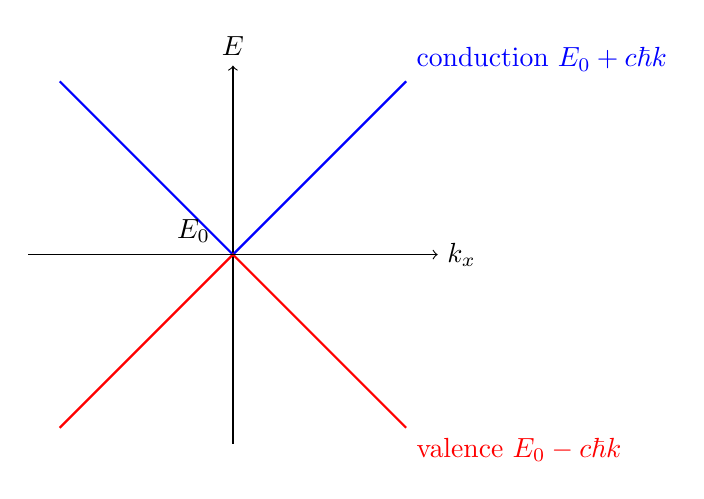
\begin{tikzpicture}[scale=1]
\draw[->] (-2.6,0) -- (2.6,0) node[right]{$k_{x}$};
\draw[->] (0,-2.4) -- (0,2.4) node[above]{$E$};
\draw[thick,blue] (-2.2,2.2) -- (0,0) -- (2.2,2.2) node[above right]{conduction $E_{0}+c\hbar k$};
\draw[thick,red]  (-2.2,-2.2) -- (0,0) -- (2.2,-2.2) node[below right]{valence $E_{0}-c\hbar k$};
\draw[dashed] (-2.6,0) -- (2.6,0);
\node at (-0.5,0.3){$E_{0}$};
\end{tikzpicture}
\end{center}

\paragraph{(ii) Comparison with a vanishing-gap parabolic semiconductor.}  Both systems have zero gap at the band-touching point and are therefore semimetallic.  The crucial differences are:
\begin{itemize}
\item \textbf{Dispersion}: linear (massless) here vs.\ quadratic (parabolic) in a conventional $E_g\to0$ semiconductor.  Carriers in the present material have an energy-independent group velocity $|\vb v_g|=c$, exactly analogous to relativistic massless particles.
\item \textbf{Density of states}: $g(E)\propto |E-E_0|$ here, vanishing linearly at the Dirac point, whereas the parabolic 2D semiconductor has $g\to\,$const there.
\item \textbf{Effective mass}: undefined (or "zero") for the linear band; finite for the parabolic case.
\item \textbf{Topology of the wavefunction}: for the linear band the eigenspinors carry a Berry phase $\pi$ around the Dirac point, leading to suppression of backscattering; the parabolic-band system does not.
\end{itemize}

\subsection*{(b) Conduction-band density}

The number of single-particle states per unit area in $k$-space is $1/(2\pi)^{2}$, with an additional factor of 2 for spin.  In a circular shell of radius $k$ to $k+dk$ the area is $2\pi k\,dk$, so the density of states per unit area as a function of energy in the conduction band ($E\ge E_{0}$) is
\begin{equation}
g(E)=2\cdot\frac{2\pi k}{(2\pi)^{2}}\,\frac{dk}{dE}=\frac{k}{\pi}\cdot\frac{1}{c\hbar}=\frac{E-E_0}{\pi c^{2}\hbar^{2}}.
\label{eq:dos}
\end{equation}
Integrating against the Fermi function $f(E)=[\,e^{\beta(E-\mu)}+1\,]^{-1}$ and substituting $u=\beta(E-E_0)$ ($du=\beta\,dE$),
\begin{align}
n_{\mathrm{el}}&=\int_{E_{0}}^{\infty}g(E)f(E)\,dE=\frac{1}{\pi c^{2}\hbar^{2}}\int_{0}^{\infty}\frac{(u/\beta)\,du/\beta}{e^{u-\alpha}+1}\nonumber\\
&=\frac{1}{\pi c^{2}\hbar^{2}\beta^{2}}\int_{0}^{\infty}\frac{u\,du}{e^{u-\alpha}+1}=\frac{1}{\pi c^{2}\hbar^{2}\beta^{2}}\cdot 1!\cdot F_{1}(\alpha),
\label{eq:nel}
\end{align}
using the definition $F_{j}(x)=(1/j!)\int_{0}^{\infty}t^{j}\,dt/(e^{t-x}+1)$.  Therefore
\begin{equation}
\boxed{\,n_{\mathrm{el}}=\frac{1}{\pi c^{2}\hbar^{2}}\,\beta^{-2}\,F_{1}(\alpha),\qquad C_{1}=\frac{1}{\pi c^{2}\hbar^{2}},\quad p=-2.\,}
\label{eq:nel-final}
\end{equation}
The $T^{2}$ behaviour mirrors the linear DOS: in 2D with a constant DOS one obtains $T^{0}$, in 2D with a linear DOS one obtains $T^{2}$.

\subsection*{(c) Conduction-band specific heat}

The electronic energy density per unit area, measured from the band edge $E_{0}$, is
\begin{equation}
\tilde u_{\mathrm{el}}=\int_{E_{0}}^{\infty}(E-E_{0})\,g(E)f(E)\,dE.
\label{eq:utilde}
\end{equation}
Using \eqref{eq:dos} and again $u=\beta(E-E_{0})$,
\begin{equation}
\tilde u_{\mathrm{el}}=\frac{1}{\pi c^{2}\hbar^{2}\beta^{3}}\int_{0}^{\infty}\frac{u^{2}\,du}{e^{u-\alpha}+1}=\frac{2}{\pi c^{2}\hbar^{2}\beta^{3}}F_{2}(\alpha)=\frac{2(k_{\mathrm B}T)^{3}}{\pi c^{2}\hbar^{2}}F_{2}(\alpha),
\label{eq:utilde2}
\end{equation}
since $F_{2}(\alpha)=\tfrac{1}{2!}\int_{0}^{\infty}u^{2}\,du/(e^{u-\alpha}+1)$.  At constant chemical potential $\mu$ (and hence constant $\tilde\mu=\mu-E_{0}$),
\begin{equation}
\frac{d\alpha}{dT}\Big|_{\mu}=\frac{d}{dT}\bigl(\tilde\mu/k_{\mathrm B}T\bigr)=-\frac{\alpha}{T}.
\label{eq:dalpha-dT}
\end{equation}
Differentiating \eqref{eq:utilde2} and using $dF_{2}/d\alpha=F_{1}$,
\begin{align}
c_{v}^{\mathrm{el}}=\frac{d\tilde u_{\mathrm{el}}}{dT}\Big|_{\mu}&=\frac{2}{\pi c^{2}\hbar^{2}}\Bigl[3 k_{\mathrm B}^{3}T^{2}F_{2}(\alpha)+(k_{\mathrm B}T)^{3}F_{1}(\alpha)\frac{d\alpha}{dT}\Bigr]\nonumber\\
&=\frac{2k_{\mathrm B}^{3}T^{2}}{\pi c^{2}\hbar^{2}}\bigl[3F_{2}(\alpha)-\alpha F_{1}(\alpha)\bigr].
\label{eq:cv-result}
\end{align}
Hence
\begin{equation}
\boxed{\,c_{v}^{\mathrm{el}}=\frac{2}{\pi c^{2}\hbar^{2}}\,k_{\mathrm B}^{3}T^{2}\bigl[3F_{2}(\alpha)-\alpha F_{1}(\alpha)\bigr],\quad C_{2}=\frac{2}{\pi c^{2}\hbar^{2}},\;q=2,\;a=3,\;b=-1.\,}
\label{eq:cv-final}
\end{equation}
The factor $\alpha F_{1}$ subtracts the energy that flows into changing the population through $\mu$: at $\tilde\mu=0$ it vanishes and the heat capacity is purely $\propto F_{2}$.

\subsection*{(d) Charge neutrality at $\tilde\mu=0$ and total specific heat}

\paragraph{(i) Equality of electron and hole numbers.}  The valence band $E=E_{0}-c\hbar k$ has DOS $g_{v}(E)=(E_{0}-E)/(\pi c^{2}\hbar^{2})$ for $E\le E_{0}$, identical in form to the conduction band reflected about $E_{0}$.  The hole occupation is $1-f(E)=[e^{\beta(\mu-E)}+1]^{-1}$.  Substituting $u=\beta(E_{0}-E)$,
\begin{equation}
n_{\mathrm{h}}=\int_{-\infty}^{E_{0}}g_{v}(E)\bigl[1-f(E)\bigr]dE=\frac{1}{\pi c^{2}\hbar^{2}\beta^{2}}\int_{0}^{\infty}\frac{u\,du}{e^{u+\alpha}+1}=\frac{F_{1}(-\alpha)}{\pi c^{2}\hbar^{2}\beta^{2}}.
\label{eq:nh}
\end{equation}
At $\tilde\mu=0$ ($\alpha=0$) we have $F_{1}(-0)=F_{1}(0)$, so $n_{\mathrm{h}}=n_{\mathrm{el}}$ identically.  By the same reflection symmetry the hole specific heat is given by \eqref{eq:cv-final} with $\alpha\to-\alpha$, equal at $\alpha=0$ to the electron contribution.

\paragraph{(ii) Total specific heat at $\tilde\mu=0$.}  Combining electron and hole contributions and setting $\alpha=0$,
\begin{equation}
c_{v}^{\mathrm{tot}}\bigr|_{\tilde\mu=0}=2\cdot\frac{2k_{\mathrm B}^{3}T^{2}}{\pi c^{2}\hbar^{2}}\cdot 3F_{2}(0)=\frac{12 k_{\mathrm B}^{3}T^{2}}{\pi c^{2}\hbar^{2}}F_{2}(0).
\label{eq:cvtot}
\end{equation}
Using the small-$\alpha$ expansion $F_{2}(\alpha)\approx 3\zeta/4+\pi^{2}\alpha/12+\tfrac{1}{2}\alpha^{2}\ln 2$ at $\alpha=0$ gives $F_{2}(0)=3\zeta/4$ with $\zeta=1.2021$.  Therefore
\begin{equation}
\boxed{\,c_{v}^{\mathrm{tot}}\bigr|_{\tilde\mu=0}=\frac{12\cdot 3\zeta/4}{\pi c^{2}\hbar^{2}}\,k_{\mathrm B}^{3}T^{2}=\frac{9\zeta\,k_{\mathrm B}^{3}T^{2}}{\pi c^{2}\hbar^{2}}.\,}
\label{eq:cvtot-final}
\end{equation}
Numerically, with $k_{\mathrm B}=\SI{1.381e-23}{J/K}$, $\hbar=\SI{1.055e-34}{J.s}$, $c=\SI{1.0e6}{m/s}$ and $T=\SI{100}{K}$:
\begin{align}
\pi c^{2}\hbar^{2}&=\pi\cdot 10^{12}\cdot (\SI{1.055e-34}{})^{2}=\SI{3.497e-56}{J^2.m^2},\\
k_{\mathrm B}^{3}T^{2}&=(\SI{1.381e-23}{})^{3}\cdot 10^{4}=\SI{2.634e-65}{J^3/K},\\
c_{v}^{\mathrm{tot}}&=\frac{9\cdot 1.2021\cdot \SI{2.634e-65}{}}{\SI{3.497e-56}{}}\approx \SI{8.15e-9}{J\,K^{-1}\,m^{-2}}.
\end{align}
This is the heat capacity per unit area of a single graphene-like layer at $\SI{100}{K}$ ($\sim\SI{8}{nJ\,K^{-1}\,m^{-2}}$); per electron it is comparable to $k_{\mathrm B}$ but the small carrier density makes the total quite small.

\subsection*{(e) Degenerate limit $\tilde\mu\gg k_{\mathrm B}T$}

Taking the given approximation $F_{2}(\alpha)\approx \alpha^{3}/6+\pi^{2}\alpha/6$ in the limit $\alpha\to\infty$, and using $F_{1}=dF_{2}/d\alpha\approx \alpha^{2}/2+\pi^{2}/6$:

\paragraph{(i) Temperature dependence of $n_{\mathrm{el}}$.} From \eqref{eq:nel-final}
\begin{equation}
n_{\mathrm{el}}=\frac{(k_{\mathrm B}T)^{2}}{\pi c^{2}\hbar^{2}}\Bigl(\tfrac{\alpha^{2}}{2}+\tfrac{\pi^{2}}{6}\Bigr)=\frac{1}{\pi c^{2}\hbar^{2}}\Bigl(\tfrac{\tilde\mu^{2}}{2}+\tfrac{\pi^{2}}{6}(k_{\mathrm B}T)^{2}\Bigr).
\label{eq:nel-degen}
\end{equation}
At leading order $n_{\mathrm{el}}=\tilde\mu^{2}/(2\pi c^{2}\hbar^{2})$, independent of $T$: the carrier density becomes the zero-temperature Fermi-volume value plus a Sommerfeld $T^{2}$ correction.

\paragraph{(ii) Chemical potential at $T\to 0$.}  Inverting the leading term of \eqref{eq:nel-degen},
\begin{equation}
\tilde\mu^{2}\to 2\pi c^{2}\hbar^{2}\,n_{\mathrm{el}}\Rightarrow \mu\to E_{0}+\hbar c\sqrt{2\pi n_{\mathrm{el}}}.
\label{eq:mu-final}
\end{equation}
Therefore
\begin{equation}
\boxed{\,C_{3}=\hbar c\sqrt{2\pi},\qquad r=\tfrac{1}{2}.\,}
\label{eq:C3r}
\end{equation}
The half-power dependence is the 2D Dirac analogue of $\mu\propto n^{2/3}$ in the 3D parabolic case and $\mu\propto n$ in the 2D parabolic case --- it follows directly from the linear DOS $g(E)\propto E$.

%================================================================
\section*{Question 4 --- Easy-axis anisotropy with transverse field, $j=1$}

\textbf{Problem statement.}  An ion of angular momentum $j$ has Hamiltonian
\[
\hat H=-D\hat J_{x}^{2}-g\mu_{\mathrm B}\hat J_{z}B,\qquad D>0,
\]
with $\hat J_{x}^{2}=\tfrac{1}{4}(\hat J_{+}^{2}+\hat J_{-}^{2})+\tfrac{1}{2}(\hat J^{2}-\hat J_{z}^{2})$.  We are asked to (a) construct the matrix representation for $j=1$ in the basis $\{\ket{1,1},\ket{1,0},\ket{1,-1}\}$, identifying $a$ and $b$; (b) diagonalise and expand to lowest order in $B$; (c) compute the partition function and transverse susceptibility and identify $f_{\perp}(D\beta)$; (d) verify limits using the given $f_{\parallel}$; (e) interpret the figure and extract $D$.

\subsection*{(a) Matrix representation in the $j=1$ basis}

In the basis $\bigl\{\ket{1,1},\ket{1,0},\ket{1,-1}\bigr\}$:
\begin{itemize}
\item $\hat J^{2}=2\hbar^{2}\,\mathbb 1$ (we set $\hbar=1$ for the matrix element coefficients).
\item $\hat J_{z}=\mathrm{diag}(1,0,-1)$, so $\hat J_{z}^{2}=\mathrm{diag}(1,0,1)$.
\item $\hat J^{2}-\hat J_{z}^{2}=\mathrm{diag}(2-1,2-0,2-1)=\mathrm{diag}(1,2,1)$.
\item $\hat J_{+}\ket{1,-1}=\sqrt{2}\ket{1,0}$ and $\hat J_{+}\ket{1,0}=\sqrt2\ket{1,1}$, so $\hat J_{+}^{2}\ket{1,-1}=2\ket{1,1}$ and $\hat J_{+}^{2}$ vanishes on the other two basis kets.  By Hermitian conjugation $\hat J_{-}^{2}\ket{1,1}=2\ket{1,-1}$.  Hence the matrix of $(\hat J_{+}^{2}+\hat J_{-}^{2})/4$ has only the (1,3) and (3,1) entries equal to $1/2$.
\end{itemize}
Adding the diagonal contribution $\tfrac12(\hat J^{2}-\hat J_{z}^{2})=\mathrm{diag}(\tfrac12,1,\tfrac12)$ gives
\begin{equation}
\hat J_{x}^{2}=\begin{pmatrix}1/2&0&1/2\\0&1&0\\1/2&0&1/2\end{pmatrix},
\label{eq:Jx2}
\end{equation}
so that the anisotropy term $-D\hat J_{x}^{2}=-D\,\mathrm{diag}\bigl[(\tfrac12,1,\tfrac12)\bigr]$ matches the form in the question with $\boxed{\,a=\tfrac{1}{2}\,}$.  The Zeeman term $-g\mu_{\mathrm B}B\hat J_{z}=-g\mu_{\mathrm B}B\,\mathrm{diag}(1,0,-1)$ then identifies $\boxed{\,b=1\,}$.

\subsection*{(b) Eigenvalues to lowest order in $B$}

The matrix $\mathsf H$ block-decomposes: the central column/row (the $\ket{1,0}$ subspace) is decoupled with eigenvalue $-D\cdot 2a=-D$ at all $B$.  The remaining $2\times 2$ block in the $\{\ket{1,1},\ket{1,-1}\}$ subspace is
\begin{equation}
\mathsf H'=\begin{pmatrix}-D/2-g\mu_{\mathrm B}B&-D/2\\-D/2&-D/2+g\mu_{\mathrm B}B\end{pmatrix}.
\label{eq:Hprime}
\end{equation}
Its trace is $-D$ and its determinant is $(D^{2}/4)-(g\mu_{\mathrm B}B)^{2}-(D/2)^{2}=-(g\mu_{\mathrm B}B)^{2}$, so the eigenvalues are
\begin{equation}
E_{\pm}=-\frac{D}{2}\pm\frac{1}{2}\sqrt{D^{2}+4(g\mu_{\mathrm B}B)^{2}}.
\label{eq:Epm-exact}
\end{equation}
For $g\mu_{\mathrm B}B\ll D$ expand the square root,
\begin{equation}
\sqrt{D^{2}+4(g\mu_{\mathrm B}B)^{2}}\approx D+\frac{2(g\mu_{\mathrm B}B)^{2}}{D},
\label{eq:sqrt-expand}
\end{equation}
so that to second order in $B$,
\begin{equation}
\boxed{\,E_{1}=+\frac{(g\mu_{\mathrm B}B)^{2}}{D},\quad E_{2}=-D,\quad E_{3}=-D-\frac{(g\mu_{\mathrm B}B)^{2}}{D}.\,}
\label{eq:E123}
\end{equation}
At $B=0$ the spectrum is $\{0,-D,-D\}$: a doublet at $-D$ (the two eigenstates of $\hat J_{x}$ with $m_{x}=\pm 1$) and a singlet at $0$ (the $m_{x}=0$ state).  A transverse field couples the two degenerate $\hat J_{z}$ eigenstates and splits the doublet quadratically; the singlet $\ket{1,0}$ is unshifted to all orders in $B$ because $\hat J_{z}\ket{1,0}=0$.

\paragraph{Sketch.} The three energies as functions of $B$:
\begin{center}
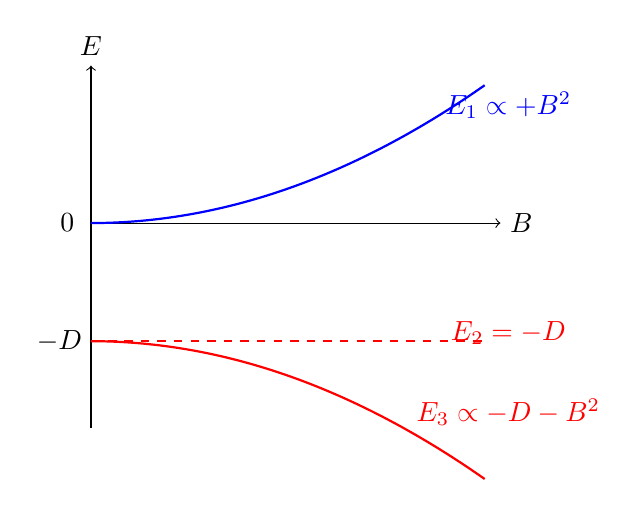
\begin{tikzpicture}[scale=1]
\draw[->] (0,0) -- (5.2,0) node[right]{$B$};
\draw[->] (0,-2.6) -- (0,2) node[above]{$E$};
\draw[domain=0:5,smooth,thick,blue] plot(\x, {0.07*\x*\x});
\draw[domain=0:5,smooth,thick,red,dashed] plot(\x,-1.5);
\draw[domain=0:5,smooth,thick,red] plot(\x, {-1.5-0.07*\x*\x});
\node[blue] at (5.3,1.5){$E_{1}\propto+B^{2}$};
\node[red]  at (5.3,-1.4){$E_{2}=-D$};
\node[red]  at (5.3,-2.4){$E_{3}\propto-D-B^{2}$};
\node at (-0.3,0){$0$};
\node at (-0.4,-1.5){$-D$};
\end{tikzpicture}
\end{center}

\subsection*{(c) Partition function and low-field transverse susceptibility}

\paragraph{(i) Partition function.}  For $N$ non-interacting ions,
\begin{equation}
Z_{N}(B)=\bigl[Z_{1}(B)\bigr]^{N},\qquad Z_{1}=e^{-\beta E_{1}}+e^{-\beta E_{2}}+e^{-\beta E_{3}}.
\label{eq:ZN}
\end{equation}
Inserting \eqref{eq:E123} and writing $w\equiv (g\mu_{\mathrm B})^{2}/D$,
\begin{equation}
Z_{1}(B)=e^{-\beta w B^{2}}+e^{\beta D}+e^{\beta D+\beta w B^{2}}.
\label{eq:Z1}
\end{equation}

\paragraph{(ii) Magnetic moment in the low-field limit.}  Expand to $O(B^{2})$:
\begin{equation}
Z_{1}(B)\approx 1+2e^{\beta D}+\beta w B^{2}\bigl(e^{\beta D}-1\bigr).
\label{eq:Z1-expand}
\end{equation}
The free energy per ion is $F_{1}=-\beta^{-1}\ln Z_{1}$, so the moment per ion is
\begin{equation}
m_{1}=-\pdone{F_{1}}{B}=\frac{1}{\beta}\,\pdone{\ln Z_{1}}{B}=\frac{2\beta w B(e^{\beta D}-1)}{1+2e^{\beta D}}\cdot \frac{1}{\beta}=\frac{2 w B(e^{\beta D}-1)}{1+2e^{\beta D}}+O(B^{3}).
\label{eq:m-ion}
\end{equation}
The total moment of the ensemble is $m=N m_{1}$.

\paragraph{(iii) Transverse susceptibility.}  By definition $\chi_{\perp}=\mu_{0}\,dm/dB|_{B\to 0}$:
\begin{equation}
\chi_{\perp}=\mu_{0}\cdot\frac{2N(g\mu_{\mathrm B})^{2}}{D}\cdot\frac{e^{\beta D}-1}{1+2e^{\beta D}}.
\label{eq:chiperp-raw}
\end{equation}
Multiplying and dividing by $\beta D/3$ to make the Curie susceptibility $\chi_{C}=2N\mu_{0}(g\mu_{\mathrm B})^{2}\beta/3$ explicit,
\begin{equation}
\chi_{\perp}=\chi_{C}\cdot\frac{3}{D\beta}\cdot\frac{e^{D\beta}-1}{1+2e^{D\beta}}.
\label{eq:chiperp-form}
\end{equation}
Hence
\begin{equation}
\boxed{\,\chi_{\perp}=\chi_{C}\,f_{\perp}(D\beta),\qquad f_{\perp}(x)=\frac{3}{x}\cdot\frac{e^{x}-1}{1+2e^{x}}.\,}
\label{eq:fperp}
\end{equation}

\subsection*{(d) Limits and inequality with the parallel case}

The reference functions are $f_{\parallel}(x)=3e^{x}/(1+2e^{x})$ and (above) $f_{\perp}(x)=(3/x)(e^{x}-1)/(1+2e^{x})$.

\paragraph{(i) Asymptotic $T\to\infty$ ($x\to 0$).}  Use $e^{x}-1\approx x$ and $1+2e^{x}\approx 3$:
\begin{align}
f_{\parallel}(0)&=3\cdot 1/3=1,\\
f_{\perp}(0)&=(3/x)\cdot x/3=1.
\end{align}
So $\chi_{\parallel},\chi_{\perp}\to\chi_{C}$ at high temperature, as expected: the anisotropy energy $D$ is negligible compared to thermal energy and the system behaves as a free $j=1$ paramagnet.

\paragraph{(ii) $\chi_{\parallel}>\chi_{C}$ at all $T$.}  We need $f_{\parallel}(x)>1$ for all $x>0$:
\begin{equation}
\frac{3e^{x}}{1+2e^{x}}>1\iff 3e^{x}>1+2e^{x}\iff e^{x}>1,
\label{eq:fpar-ineq}
\end{equation}
which holds for all $x>0$. Thus $\chi_{\parallel}>\chi_{C}$.  Physically, when the field is along the easy axis, the lowest two states $\ket{m_{x}=\pm1}$ are split linearly in $B$, so the population imbalance grows faster than for a free spin and the susceptibility is enhanced.

\paragraph{(iii) $\chi_{\perp}$ finite at $T=0$.}  In the low-temperature limit $x\to\infty$, $e^{x}-1\sim e^{x}$ and $1+2e^{x}\sim 2e^{x}$, so
\begin{equation}
\chi_{\perp}\to 2N\mu_{0}(g\mu_{\mathrm B})^{2}/D\cdot \tfrac{1}{2}=\frac{N\mu_{0}(g\mu_{\mathrm B})^{2}}{D}.
\label{eq:chiperp-zeroT}
\end{equation}
This is finite --- a Van Vleck-type response.  Mechanism: with the field perpendicular to the easy axis, the ground states $\ket{m_{x}=\pm1}$ have $\langle\hat J_{z}\rangle=0$ but the field admixes them with the $\ket{m_{x}=0}$ excited state at energy $D$ above; second-order perturbation theory gives a $B$-linear induced moment whose coefficient is independent of temperature once $k_{\mathrm B}T\ll D$.  In contrast $\chi_{C}\propto 1/T$ diverges, so $f_{\perp}(x)=\chi_{\perp}/\chi_{C}\to 0$ at $T=0$ even though $\chi_{\perp}$ itself does not.

\subsection*{(e) Interpretation of the figure and determination of $D$}

\paragraph{Physical picture.}  The plot shows three molar susceptibilities for $g=2$ as functions of temperature.  At high $T$ (\textgreater\,$25$~K) all three converge to a single curve, the Curie tail, because $k_{\mathrm B}T\gg D$ and the ion behaves isotropically.  At low $T$ the anisotropy splits the response: $\chi_{\parallel}$ is a factor $3/2$ larger than $\chi_{C}$ (because $f_{\parallel}\to 3/2$ as $x\to\infty$) but still diverges as $1/T$, while $\chi_{\perp}$ saturates at the Van Vleck value $N_{A}\mu_{0}(g\mu_{\mathrm B})^{2}/D$.  This is the classic behaviour of a single-ion easy-axis anisotropy with the field along ($\parallel$) or transverse to ($\perp$) the anisotropy axis.

\paragraph{Extracting $D$.}  Reading off the saturation value of $\chi_{\perp}$ at $T\to 0$ from the figure, $\chi_{\perp}^{\mathrm{sat}}\approx \SI{3e-6}{m^{3}/mol}$, and equating to the Van Vleck expression,
\begin{equation}
\frac{N_{A}\mu_{0}(g\mu_{\mathrm B})^{2}}{D}=\chi_{\perp}^{\mathrm{sat}}\Rightarrow D=\frac{N_{A}\mu_{0}(g\mu_{\mathrm B})^{2}}{\chi_{\perp}^{\mathrm{sat}}}.
\label{eq:D-extract}
\end{equation}
With $N_{A}=\SI{6.022e23}{mol^{-1}}$, $\mu_{0}=\SI{1.2566e-6}{H/m}$, $g=2$, $\mu_{\mathrm B}=\SI{9.274e-24}{J/T}$:
\begin{align}
N_{A}\mu_{0}(g\mu_{\mathrm B})^{2}&=6.022\times 10^{23}\cdot 1.2566\times 10^{-6}\cdot (\SI{1.855e-23}{})^{2}\nonumber\\
&=6.022\times 10^{23}\cdot 1.2566\times 10^{-6}\cdot 3.441\times 10^{-46}\nonumber\\
&\approx \SI{2.604e-28}{J\,m^{3}/mol},
\end{align}
hence
\begin{equation}
D\approx \frac{\SI{2.604e-28}{J\,m^{3}/mol}}{\SI{3e-6}{m^{3}/mol}}=\SI{8.7e-23}{J}\approx k_{\mathrm B}\cdot \SI{6.3}{K}.
\label{eq:D-numerical}
\end{equation}
Equivalently $D/k_{\mathrm B}\approx 6$~K, consistent with the temperature at which the figure shows the three curves diverging from each other.
\begin{equation}
\boxed{\,D\approx \SI{8.7e-23}{J}\;\;(\,D/k_{\mathrm B}\approx \SI{6}{K}\,).\,}
\label{eq:D-final}
\end{equation}
A useful internal consistency check: the curves visibly merge once $T\gtrsim 4 D/k_{\mathrm B}\approx \SI{25}{K}$, which matches the regime where $f_{\perp}\approx f_{\parallel}\approx 1$, exactly as found in part (d)(i).

\end{document}
